\documentclass{article}
\usepackage{amsmath} % need to be on top for eps files
\usepackage{graphicx}
\graphicspath{ {/images/} }
%set the relative location for eps files

\usepackage[utf8]{inputenc}
\usepackage{amsmath}%To be able to use split in equation
\usepackage{datatool,siunitx}
\usepackage{float}
\usepackage{url}

%Working solution Table aligned left
\usepackage{array}
\newcolumntype{L}[1]{>{\raggedright\let\newline\\\arraybackslash\hspace{0pt}}m{#1}}
\newcolumntype{C}[1]{>{\centering\let\newline\\\arraybackslash\hspace{0pt}}m{#1}}
\newcolumntype{R}[1]{>{\raggedleft\let\newline\\\arraybackslash\hspace{0pt}}m{#1}}

\usepackage{enumitem} % enumerate alphabetically

% Attempt 0
%\usepackage{enumitem,tabularx,showframe,calc}
% Attempt 1
%\usepackage{ragged2e,array}
% Attempt 2-4
%\usepackage{tabularx}

%Attempt 7
\usepackage{tabularx}
\usepackage{booktabs}
\usepackage{caption}

% To get mutliple  columns:{
\usepackage{multicol}
% To get clever references, used in this example.
\usepackage{cleveref} %cleverref needs to stand below amsmath package.
% }
% To get side by side pictures:{
\usepackage{caption}
\usepackage{subcaption}
\usepackage{graphicx}

% }

%%%%%%%%%%% to rotate figures and make them full page:
\usepackage{graphicx}
\usepackage{enumitem}
\usepackage{wrapfig}
\usepackage{lscape}
\usepackage{rotating}
\usepackage{epstopdf}

% to add a full A4 size gantt chart picture
\usepackage{pdfpages} 

%%%%%%% GET SIDE BY SIDE IMAGES
\usepackage{subfig}


%Get straigth quotation marks:
\usepackage{textcomp}
\usepackage[T1]{fontenc}  % access \textquotedbl
\usepackage{textcomp}     % access \textquotesingle
\usepackage{mathptmx}     % load "Times New Roman" text font 
                          % (note: the "times" package is obsolete!)
                          
                          
%%%%%%%%%%%%%%% Add lemaas and proofs
\usepackage{amsthm}
\usepackage{blindtext}
\usepackage{amssymb}
\usepackage{amsthm}

%\newtheorem{theorem}{Theorem}
\newtheorem{theorem}{Theorem}[section]
\newtheorem{corollary}{Corollary}[theorem]
\newtheorem{lemma}[theorem]{Lemma}

\theoremstyle{remark}
\newtheorem*{remark}{Remark}

\theoremstyle{definition}
\newtheorem{definition}{Definition}[section]
%%%%%%%%%%%%%%% Add lemaas and proofs

% %%%%%%%%%%%%%%%%%%%%% add theorems with auto section numbering
% \theoremstyle{plain}
% \newtheorem{thm}{Theorem}[section]
% \newtheorem{lem}[thm]{Lemma}
% \newtheorem{prop}[thm]{Proposition}
% \newtheorem*{cor}{Corollary}

% \theoremstyle{definition}
% \newtheorem{defn}{Definition}[section]
% \newtheorem{conj}{Conjecture}[section]
% \newtheorem{exmp}{Example}[section]

% \theoremstyle{remark}
% \newtheorem*{rem}{Remark}
% \newtheorem*{note}{Note}
% %%%%%%%%%%%%%%%%%%%%% add theorems

%%%%%%%%%%%%Create custom theorem numbering:
\newtheorem{innercustomthm}{Theorem}
\newenvironment{customthm}[1]
  {\renewcommand\theinnercustomthm{#1}\innercustomthm}
  {\endinnercustomthm}
%%%%%%%%%%%%Create custom theorem numbering:





%%%%%%%%%%%%%%%%%%%%%%%%%%%%%%%%%%%%%%%% Create listings (Java)
\usepackage{listings}
\usepackage{color}

% Source: https://www.overleaf.com/project/5ca8e08c504f2453fce240ba
\definecolor{mygreen}{rgb}{0,0.6,0}
\definecolor{mygray}{rgb}{0.5,0.5,0.5}
\definecolor{mymauve}{rgb}{0.58,0,0.82}

\lstset{ %
  backgroundcolor=\color{white},   % choose the background color
  basicstyle=\footnotesize,        % size of fonts used for the code
  breaklines=true,                 % automatic line breaking only at whitespace
  captionpos=b,                    % sets the caption-position to bottom
  commentstyle=\color{mygreen},    % comment style
  escapeinside={\%*}{*)},          % if you want to add LaTeX within your code
  keywordstyle=\color{blue},       % keyword style
  stringstyle=\color{mymauve},     % string literal style
}

%%%% Auto generate table from CSV%%%%%
% \usepackage{booktabs} % For \toprule, \midrule and \bottomrule
% \usepackage{siunitx} % Formats the units and values
% \usepackage{pgfplotstable} % Generates table from .csv

% % Setup siunitx:
% \sisetup{
%   round-mode          = places, % Rounds numbers
%   round-precision     = 2, % to 2 places
% }

\usepackage{csvsimple}
\usepackage{geometry}
 \geometry{
 a4paper,
 total={175mm,265mm},
 left=15mm,
 top=15mm,
 }

\usepackage{cleveref} %cleverref needs to stand below amsmath package.
\crefname{lstlisting}{listing}{listings}
\Crefname{lstlisting}{Listing}{Listings}



\title{Technical examples}
\author{A-T-0}
\date{April 2018}

%%%%
% use with cleveref
% also copy text of appsec in the main body that contains appsec with the actual ref to appendices.tex
\usepackage{appendix}
\crefname{appsec}{Appendix}{Appendices} % refer to appendix as appendix iso as section
\begin{document}

\maketitle
\tableofcontents

\newpage
\section{Introduction}



\subsection{Importing/synchronizing variables with latex}
\begin{enumerate}
    \item include package: usepackage{listings} %Allows import of lists (withs specific lines)
    \item create .txt file with every value you want somewhere (in an equation) on a separate line
    \item Add description of variable in the line above that variable, and (line)-number that description
    \item create a folder in your latex working environment, e.g. named: $"data\_input"$
    \item upload e.g. "test.txt" with the variables and descriptions
    \item To input the parameter in latex use the following line:
    %\lstinputlisting[firstline=2,lastline=2]{data_input/test.txt}
    \item Party!
\end{enumerate}

\subsection{Importing/synchronizing variables with latex V1.0}
    \begin{enumerate}
    \item add the package listed in the comment, then add the lines below the comment
%\usepackage{datatool,siunitx}
    \item Then upload the .txt file that contains the variables.

\DTLloaddb[noheader]{data}{testfile.txt}
\newcommand{\mydatavalue}[1]{%
  \begingroup
  \dtlgetrow{data}{#1}%
  \dtlgetentryfromcurrentrow{\temp}{1}%
  \num{\temp}%
  \endgroup
}
    \item and call it with 
    \item $K_{sh} = \mydatavalue{2}$
    \item $K_{sh} = \mydatavalue{4}$
\end{enumerate}
\section{Reducing subsection spacing}

% \usepackage{titlesec}

% \titlespacing\section{0pt}{12pt plus 4pt minus 2pt}{0pt plus 2pt minus 2pt}
% \titlespacing\subsection{0pt}{12pt plus 4pt minus 2pt}{0pt plus 2pt minus 2pt}
% \titlespacing\subsubsection{0pt}{12pt plus 4pt minus 2pt}{0pt plus 2pt minus 2pt}
\subsection{reducing white border margins on edges sides of page}
% fit text to page
% \usepackage{geometry}
% \geometry{legalpaper, portrait, margin=0.5in}
\newpage
% How to generate a table with automatically wrapped text:
\section{How to generate a table with automatically wrapped text}
\subsection{And how to shift table left}
*the hspace shifts the table left
% \documentclass{article}

% \usepackage{array}
% \newcolumntype{L}[1]{>{\raggedright\let\newline\\\arraybackslash\hspace{0pt}}m{#1}}
% \newcolumntype{C}[1]{>{\centering\let\newline\\\arraybackslash\hspace{0pt}}m{#1}}
% \newcolumntype{R}[1]{>{\raggedleft\let\newline\\\arraybackslash\hspace{0pt}}m{#1}}

%\begin{document}
    This is a working example of a wrapped text table where the text is left-aligned without the text in the cells being all smeared out.
    \begin{table}[H]
    %\begin{tabular}{|l|l|l|l|l|l|l|}
    \hspace*{-11.50em}
    %\begin{tabular}{|p{3cm}|p{3cm}|p{2.5cm}|p{2cm}|p{2.cm}|p{2.cm}|p{2.cm}|}
    \begin{tabular}{| L{3cm} |L{3cm}|L{2.5cm}|L{2cm}|L{2.cm}|L{2.cm}|L{2.cm}|}
    \hline
    Week2Lecture2 ANN: Perceptrons, MLP and Backpropagation &   1. 1.a. Neural Networks Supervised  &   2. 1.b. Neural Networks UnSupervised    &   9. 5.a. Notation    &       &       &       \\ \hline
    W2L3 ANN: Training and building MLPs    &   1. 1.a. Neural Networks Supervised  &   2. 1.b. Neural Networks UnSupervised    &   12. 5.d Gradient descent    &   13. 5.e Training Neural Networks    &   10. 5.b. Model Architecture &   11. 5.c Loss Function   \\ \hline
    W3L4 Reinforcement Learning &   4. 2.a. Reinforcement Learning  &       &       &       &       &       \\ \hline
    W3L5 Genetic Algorithms &   3. 1.c Evolutionairy Computing  &   5. 3.a. Evolutionairy computing &       &       &       &       \\ \hline
    W4L6 Swarm Intelligence &   6. 3.b. Swarm Intelligence  &       &       &       &       &       \\ \hline
    W4L7 CI Math and Principles Overview    &   9. 5.a. Notation    &   7. 3.c Bayesian Reasoning   &       &       &       &       \\ \hline
    W5L8 ANN: Unsupervised  &   2. 1.b. Neural Networks UnSupervised    &       &       &       &       &       \\ \hline
    W5L9 ANN: Deep/Recurrent and Gradient Descent   &   12. 5.d Gradient descent    &   4. 2.a. Reinforcement Learning  &   11. 5.c Loss Function   &       &       &       \\ \hline
    W6L10 Evolutionary Strategies, Genetic Programming  &   5. 3.a. Evolutionairy computing &   3. 1.c Evolutionairy Computing  &       &       &       &       \\ \hline
    W6L11 Mixed CI strategies   &   All &       &       &       &       &       \\ \hline
    W6L12 (Werkcollege) Swarm routing   &   6. 3.b. Swarm Intelligence  &       &       &       &       &       \\ \hline
    \end{tabular}
    \end{table}
%\end{document}
% \end{document}

\newpage
%\usepackage{multicol}

\section{Mutlicolumns}
\begin{multicols}{2}
For low epsilon (illustrated in \cref{fig:toy_maze_low_epsilon} and \cref{fig:easy_maze_low_epsilon}):
    \begin{enumerate}
        \item A steeper slope downwards and/or a more convergent solution  downwards is observed towards the end (trials 7 to 10). %graph 1
        \item A steeper slope is found at the start of the learning trials (2 to 4), but the slope is levelled after the first 2 trials. %graph 1 Graph 4.
    \end{enumerate}

\columnbreak
For a higher epsilon (illustrated in \cref{fig:toy_maze_high_epsilon} and  \cref{fig:easy_maze_high_epsilon}):
    \begin{enumerate}
        \item A steeper learning rate is found in trials 4/5 to 6/7. %graph 8 and 7
        \item A less steep downwards slope is found towards the end of the trials (7-10). %graph7 8 and 7
        \item More variation in the number of steps during the final trials 7-10 is found. %sortof graph7weak 7 and 8 +Easy 9
        \item The generally, the absolute number of steps after 10 trials, is lower for a higher learning rate.
    \end{enumerate}
\end{multicols}



\section{Multiple figers next to eachother}
Enter the following text above main:
\begin{verbatim}
    % To get side by side pictures:{
\usepackage{caption}
\usepackage{subcaption}
\usepackage{graphicx}
\end{verbatim}

\begin{figure}[H]
\centering
\begin{subfigure}{.48\textwidth}
  \centering
  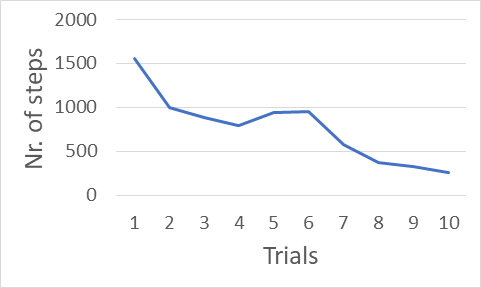
\includegraphics[width=0.99\linewidth]{images/2.2training/1Graph3.png}
    \caption{Toy maze with $\epsilon = 0.1$}
    \label{fig:toy_maze_low_epsilon}
\end{subfigure}
\begin{subfigure}{.48\textwidth}
  \centering
  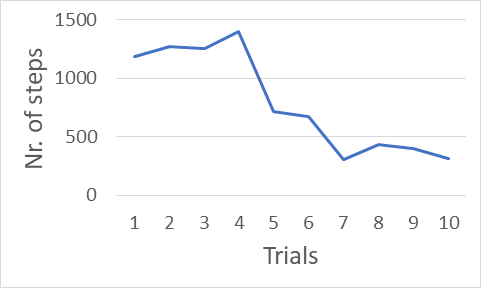
\includegraphics[width=1\linewidth]{images/2.2training/7Graph3.png}
      \caption{Toy maze with  $\epsilon = 0.7$}
    \label{fig:toy_maze_high_epsilon}
\end{subfigure}
%\label{fig:perceptron_learning_performance}
\begin{subfigure}{.48\textwidth}
  \centering
  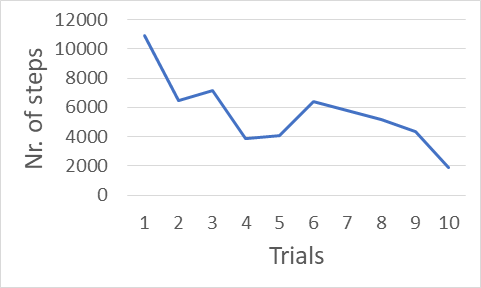
\includegraphics[width=0.99\linewidth]{images/2.2training/0Graph4.png}
    \caption{Easy maze with $\epsilon = 0.1$}
    \label{fig:easy_maze_low_epsilon}
\end{subfigure}
\begin{subfigure}{.48\textwidth}
  \centering
  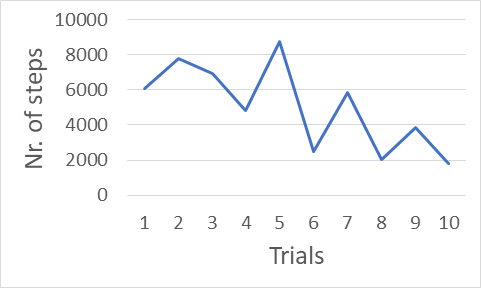
\includegraphics[width=1\linewidth]{images/2.2training/9Graph4.png}
      \caption{Easy maze with $\epsilon = 0.9$}
    \label{fig:easy_maze_high_epsilon}
\end{subfigure}
\caption{Number of steps required for robot to reach target with learning, as a function of $\epsilon$.}
%\label{fig:perceptron_learning_performance}
\end{figure}


\section{Evend out columns:}
\begin{multicols}{2}
\noindent Low $\epsilon$ advantage(s): 
    \begin{itemize}
        \item A quick decrease in initial required number of steps at the start of agent learning trials.
        \item A higher rate of conversion to the optimal solution, once it has been learned, due to a lower exploration rate
    \end{itemize}
\noindent Low $\epsilon$ disadvantage(s):
\begin{itemize}
    \item A plateau due to a lower initial exploration of options
    \item Higher risk of getting stuck in a "local minimum" due to reduced rate of exploration.
\end{itemize}
\columnbreak
High $\epsilon$ advantage(s): 
\cref{fig:easy_maze_high_epsilon}):
    \begin{itemize}
        \setcounter{enumi}{2}
        \item An increased chance of finding the actual optimum route in stead of a local minimum, due to the increased rate of exploration.
    \end{itemize}
\bigskip
\bigskip
\bigskip
\bigskip
\bigskip
\bigskip
\bigskip
\bigskip
\noindent High $\epsilon$ disadvantage(s): 
\begin{itemize}
    \item A slower rate of "learning/performance improvement" due to inital higher rate of exploration.
    \item Lower convergence to the final optimal solution once it has been learned, due to increased exploration.
\end{itemize}
\end{multicols}

\setcounter{section}{1} 
\setcounter{subsection}{1}
\section{Custom subsection and enumeration numbering}
\begin{enumerate}
    \setcounter{enumi}{4} 
    \item Start
    \item last enumeration
\end{enumerate}
\subsection{alphanumeric numbering}
Use package \verb+\usepackage{enumitem}\verb+
\begin{enumerate}[label=(\alph*)]
    \item Start
    \item last enumeration
\end{enumerate}

\subsection{Alhpanumeric subsections}
\renewcommand{\thepart}{\Alph{part}}
%\renewcommand{\thechapter}{\Roman {chapter}}
\renewcommand{\thesection}{\arabic{section}}
\renewcommand{\thesubsection}{\alph{subsection})}
\renewcommand{\thesubsubsection}{\alph{subsection}\alph{subsubsection})}
\section{Weird symbols}
\subsection{Straight quotes}
sometext \textquotedbl sometext\textquotedbl
\subsection{dollarsign}
sometext\$ sometext 
\subsection{Percentage sign}
Sometext\%Sometext
\subsection{\&}
\subsection{force a space}
Somespace \: somespace
\subsection{Dash wave~}
\textasciitilde
\subsection{Streepje=hyphen}
\subsection{non-numbered equation}
\subsection{Symbol: sum}
\subsection{Adapting equation brackets}
\begin{equation*}
\sum_{i=1}^n i = \left(\sum_{i=1}^{n-1} i\right) + n =
\frac{(n-1)(n)}{2} + n = \frac{n(n+1)}{2}
\end{equation*}
\subsection{Sybmol: is part of, and sum}
\begin{equation}
\sum_{i=1}^n i = \in a
\end{equation}
\subsection{Writing tow things below eachother as fraction without the dash:}
\begin{equation}
    \underset{a}{min} 
\end{equation}
\subsection{Custom equation numbering}
\begin{equation}
    R_n^E=\sum_{t=1}^{n}l_m(p_t,z_t)-{\underset{i}{min}} \sum_{t=1}^{n}{z_t}^i
    \tag{-3444asdf234234}
    \label{eq:expert_ragrats}
\end{equation}
\section{equations}
\subsection{Splitting equations over multiple lines}
Keywords: split, equation, multiple lines, vspace, line space, enter
\begin{equation}
    \begin{split}
    rad_{worst} \cdot K_{shielding}^n = 3 \\
    rad_{best} \cdot K_{shielding}^n = 3 \\
    817308 \cdot {\frac{1}{2}}^n = 3 \\
    81730.8 \cdot {\frac{1}{2}}^n = 3
    \end{split}
    \label{eq:shield_factor}
\end{equation}

 \[ x+y = \begin{cases} \mbox{true,} & \mbox{if } 0 < x < 5 \\ \mbox{false,} & \mbox{otherwise} \end{cases} \]
\subsection{Matrices}
%\usepackage{amsmath}
\[
\begin{bmatrix}
    x_{11}       & x_{12} & x_{13} & \dots & x_{1n} \\
    x_{21}       & x_{22} & x_{23} & \dots & x_{2n} \\
    \hdotsfor{5} \\
    x_{d1}       & x_{d2} & x_{d3} & \dots & x_{dn}
\end{bmatrix}
=
\begin{bmatrix}
    x_{11} & x_{12} & x_{13} & \dots  & x_{1n} \\
    x_{21} & x_{22} & x_{23} & \dots  & x_{2n} \\
    \vdots & \vdots & \vdots & \ddots & \vdots \\
    x_{d1} & x_{d2} & x_{d3} & \dots  & x_{dn}
\end{bmatrix}
\]

Or just a single matrix:
\begin{equation}
\begin{bmatrix}
    x_{1}       & 1 & sin(2\pi x_1) & cos(2\pi x_1)\\
    x_{2}       & 1 & sin(2\pi x_2) & cos(2\pi x_2)\\
    \hdotsfor{3} \\
    x_{n}       & 1 & sin(2\pi x_n) & cos(2\pi x_n)\\
\end{bmatrix}
    \label{eq:h_matrix_q1b}
\end{equation}
\section{proof:}
\theoremstyle{plain}

% automatic section numbering theorem



% %%%%%%%%%%%%Create custom theorem numbering:
% \newtheorem{innercustomthm}{Theorem}
% \newenvironment{customthm}[1]
%   {\renewcommand\theinnercustomthm{#1}\innercustomthm}
%   {\endinnercustomthm}
% %%%%%%%%%%%%Create custom theorem numbering:
\begin{customthm}{99}[Somebody]\label{ninetynine}
Statement.
\end{customthm}

%So all theorems must be custom numbered
\begin{customthm}[]\label{ninetynine}
Statement.
\end{customthm}


\begin{lemma}
To prove: $L(m_-,m_+,a)$ is a convex on its domain $\mathbb{R}^d \times \mathbb{R}^d \times \mathbb{R}$.
\end{lemma}
 
\begin{proof}
Using a direct proof, a norm is proved to be convex. The variables of the function $L$ are added and combined using only operations that preserve convexity until it equals function $L$. 
\\
Starting with a mapping $f\rightarrow ||f||$,$f\in V$,  $||f|| \in \mathbb{R^d}$, function $f$is a norm by definition 2.2 of \cite{norm_definition} if the following conditions hold:
\begin{equation}
    \forall a \in V:||a||\geq
    \label{eq:convex0}
\end{equation}
\begin{equation}
    ||a||=0 \Leftrightarrow a=0
    \label{eq:convex1}
\end{equation}
\begin{equation}
    \forall a \in V, \lambda \in \mathbb{R}:\lambda||a||=||\lambda a||
    \label{eq:convex2}
\end{equation}
\begin{equation}
    \forall a,b\in V:||a+b||\leq ||a||+||b||
    \label{eq:convex3}
\end{equation}
Using the definition of convex\cite{zinkevich2003online}, a function $f:V\rightarrow \mathbb{R}$ is convex if:
\begin{equation}
    a,b \in V,\lambda \in[0,1]:f(\lambda a+(1-\lambda)b)\leq \lambda f(a)+(1-\lambda)f(b)
    \label{eq:convex4}
\end{equation}
%v,w∈V,λ∈[0,1]:f(λv+(1−λ)w)≤λf(v)+(1−λ)f(w)
Since $\lambda \in [0,1]$, \cref{eq:convex2} can be used to move $\lambda$ out, and \cref{eq:convex3} can be used to separate the terms $a$ and $(1-\lambda)$. That yields \cref{eq:convex5} and \cref{eq:convex6} for norm $||f(a,b,\lambda)||$ in $\mathbb{R}$.

\begin{equation}
    ||\lambda a+(1-\lambda)b||\leq ||\lambda a||+||(1-\lambda)b||
    \label{eq:convex5}
\end{equation}
with:
\begin{equation}
    ||\lambda a||+||(1-\lambda)b||=\lambda||a||+(1-\lambda)||w||
    \label{eq:convex6}
\end{equation}

That proves norm $||f(a,b,\lambda)||$ is convex in $\mathbb{R}$. This norm is rewritten twice, both to the $l_1$-norm. However, that requires the domain $f \in \mathbb{R}$ to be mapped to $f \in \mathbb{R^4}$. For that purpose, convexity preserving operation $f:\mathbb{R^n}\rightarrow \mathbb{R^m}$ of slide 9 of \cite{preserving_convexity} is used.

Next, the variables of general norm $||f||$ are substituted. $a$ is substituted by $m_+$,$b$ by $m_-$, $\lambda$ by $a$. Multiplying by $\lambda_1$ to create the right term of $L$:
\begin{equation}
    \lambda_1||m_+-m_-+a||_1
    \label{eq:convex7}
\end{equation}
For the second term, $a$ is substituted by $x_i^c$, $b$ with $m_c$ yielding:
\begin{equation}
    ||x_i^c-m_c||_1 
    \label{eq:convex8}
\end{equation}

The elements of the double summation of norm \cref{eq:convex8} and norm \cref{eq:convex9} are added using the weighted summation with $w_i=1$ of rule 1 of convexity preserving rules by \cite{preserving_convexity_rules_berkely}.

That proves
\begin{equation}
    L(m_-,m_+,a):=\left(\sum_{c \in \{-,+\}}^j \sum_{i}^{N_c}||x_i^c-m_c||_1 \right)+\lambda ||m_+m_-+a||_1
    \label{eq:objective_function}
\end{equation}

is convex in it's domain $\mathbb{R}^d\times \mathbb{R}^d \times \mathbb{R}$
\end{proof}
\section{How to properly enter code listings of any language}
Source: \url{https://www.overleaf.com/project/5ca8e08c504f2453fce240ba}

First add the commented code to the main, above begin document. Then add the listing in the folder listing, and then you can add the listing as is done in \cref{lst:value_iteration}.



\lstinputlisting[language=java,caption={myListing},label={lst:value_iteration}]{listings/listingExample.java}

\subsection{Matlab listing}
% % Create a matlab listing
% \usepackage{listings}
% \usepackage{color} %red, green, blue, yellow, cyan, magenta, black, white
% \definecolor{mygreen}{RGB}{28,172,0} % color values Red, Green, Blue
% \definecolor{mylilas}{RGB}{170,55,241}

Then inside \verb+begin documetn+:
\begin{verbatim}
\begin{document}

% Specify matlab listing style
\lstset{language=Matlab,%
    %basicstyle=\color{red},
    breaklines=true,%
    morekeywords={matlab2tikz},
    keywordstyle=\color{blue},%
    morekeywords=[2]{1}, keywordstyle=[2]{\color{black}},
    identifierstyle=\color{black},%
    stringstyle=\color{mylilas},
    commentstyle=\color{mygreen},%
    showstringspaces=false,%without this there will be a symbol in the places where there is a space
    numbers=left,%
    numberstyle={\tiny \color{black}},% size of the numbers
    numbersep=9pt, % this defines how far the numbers are from the text
    emph=[1]{for,end,break},emphstyle=[1]\color{red}, %some words to emphasise
    %emph=[2]{word1,word2}, emphstyle=[2]{style},    
}    
\end{verbatim}

\section{Figures}

\subsection{Side by side images}
%\usepackage[demo]{graphicx}
%\usepackage{subfig}

\begin{figure}[H]
\centering
\parbox{5cm}{
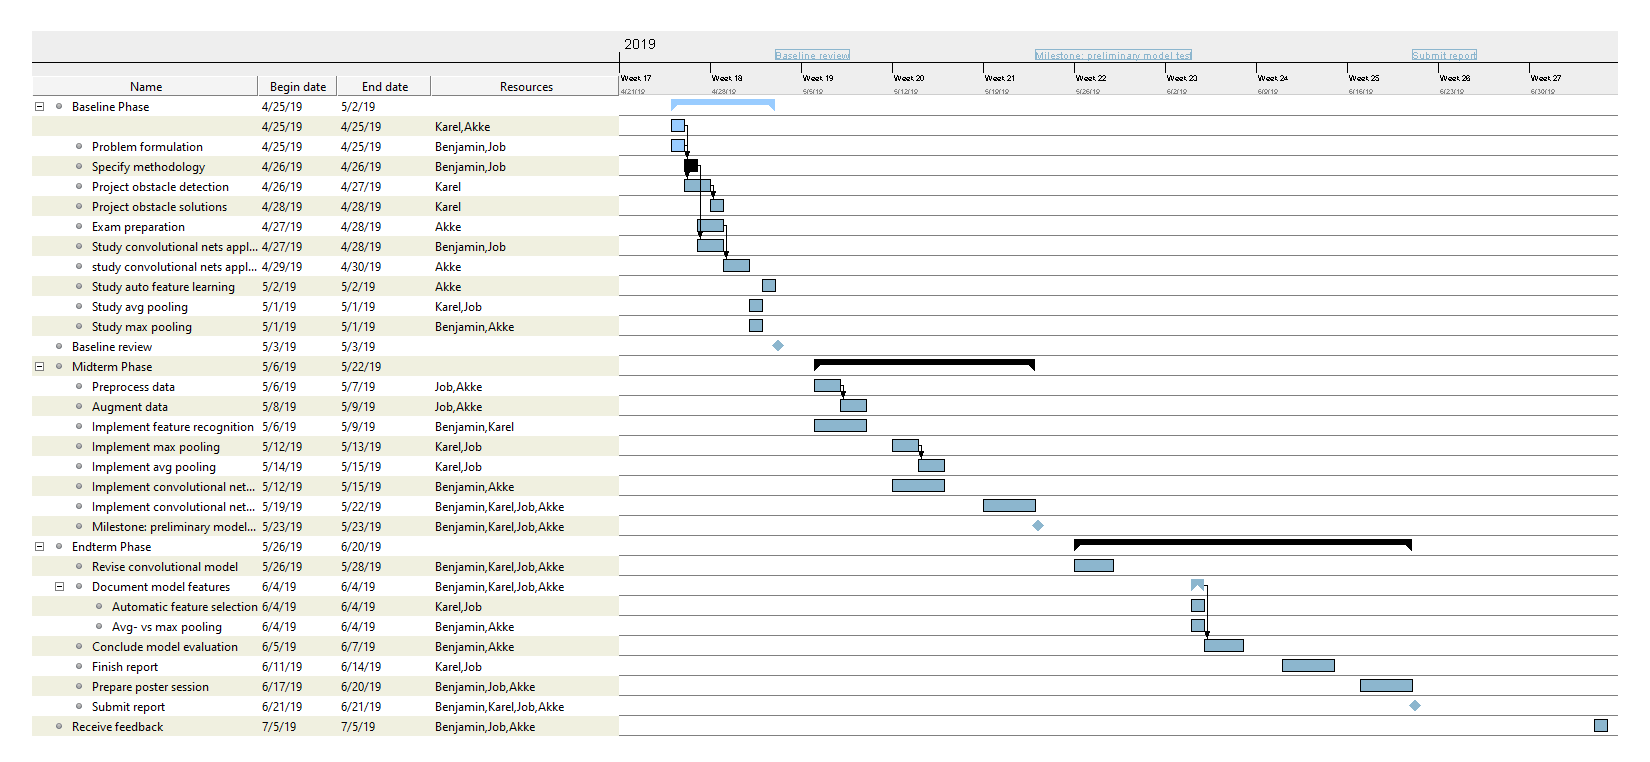
\includegraphics[width=5cm]{images/ganttV4horizontal.png}
\caption{First.}
\label{fig:2figsA}}
\qquad
\begin{minipage}{5cm}
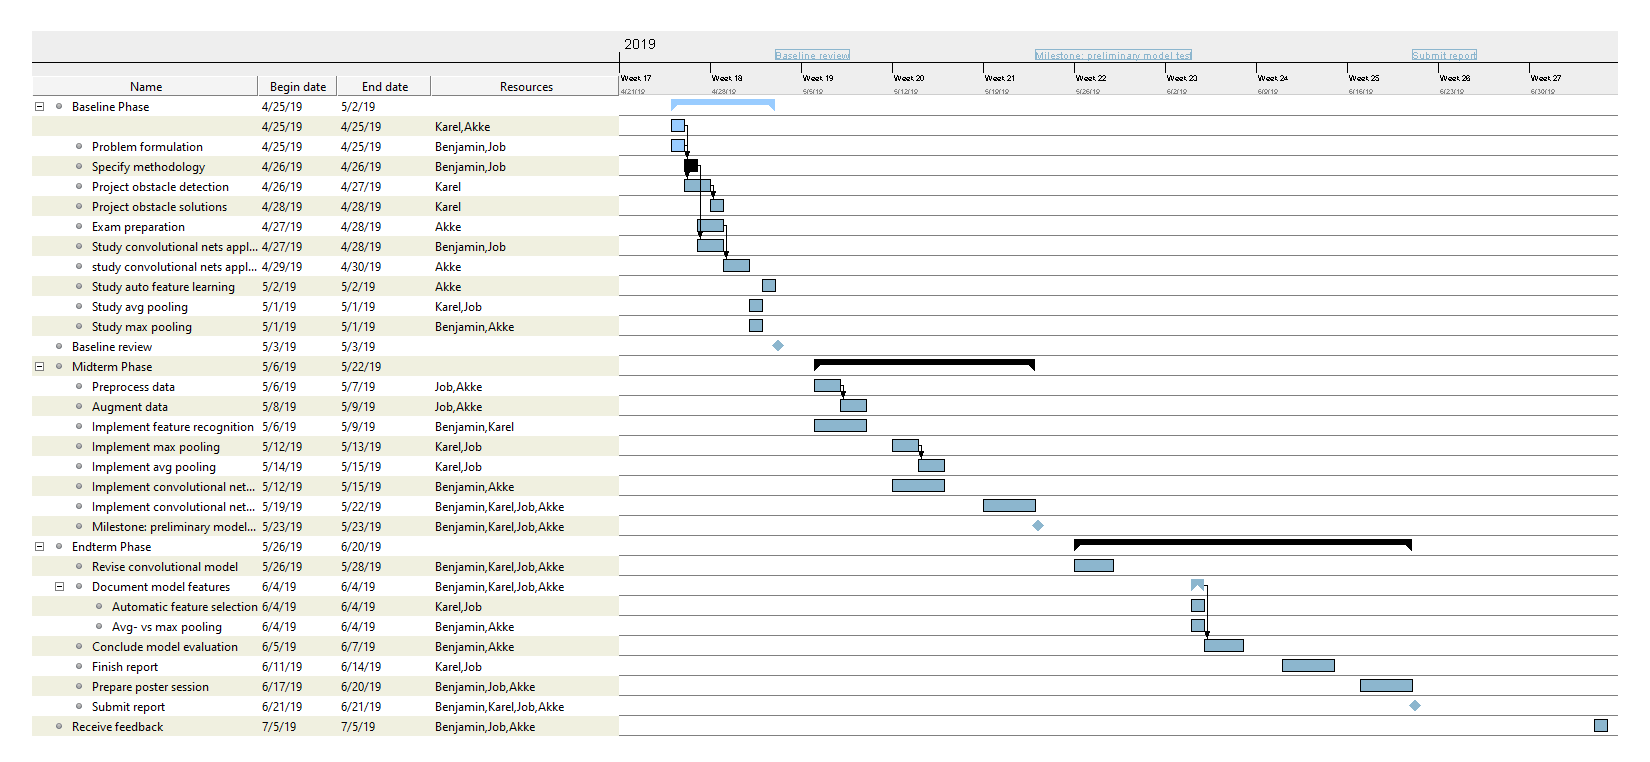
\includegraphics[width=5cm]{images/ganttV4horizontal.png}
\caption{Second.}
\label{fig:2figsB}
\end{minipage}
\end{figure}



%\usepackage{enumitem}
\subsection{Wrap enumeration around figure:}
  {\bfseries Multiple Choice: }% do not use \bf in LaTeX it is deprecated 20+ years ago
  \begin{enumerate}
    \item As shown in the figure. This rock is phaneritic and contains quartz, K-feldspar, and plagioclase in nearly equal amounts. What is it?

    \begin{minipage}{.45\textwidth}
      \begin{enumerate}[label=(\Alph*), itemsep=0pt]% never number things manually!
        \item rhyolite
        \item basa
        \item diorite
        \item ash-flow tuff
        \item  granite
      \end{enumerate}
    \end{minipage}
    \begin{minipage}{.45\textwidth}
      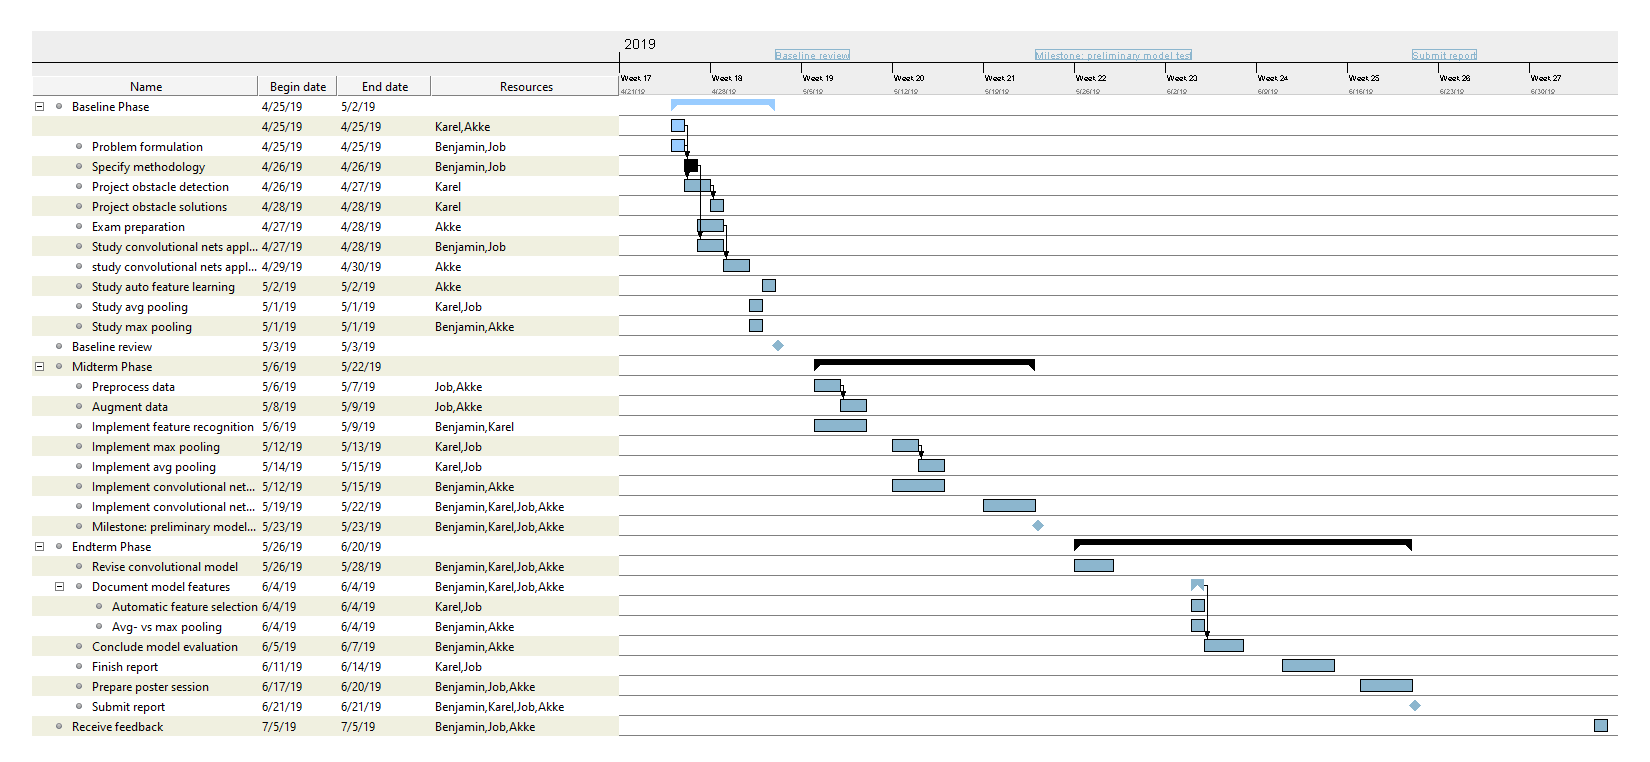
\includegraphics[scale=0.1]{images/ganttV4horizontal.png}
    \end{minipage}
  \end{enumerate}



\subsection{full page horizontal figure with caption}

% \begin{comment}
% % rotate picture attempt 4
% \usepackage{graphicx}
% \usepackage{wrapfig}
% \usepackage{lscape}
% \usepackage{rotating}
% \usepackage{epstopdf}

% \usepackage{graphicx}
% \graphicspath{ {./} }
% \end{comment}

\begin{sidewaysfigure}[ht]
\hspace*{-4cm}   
    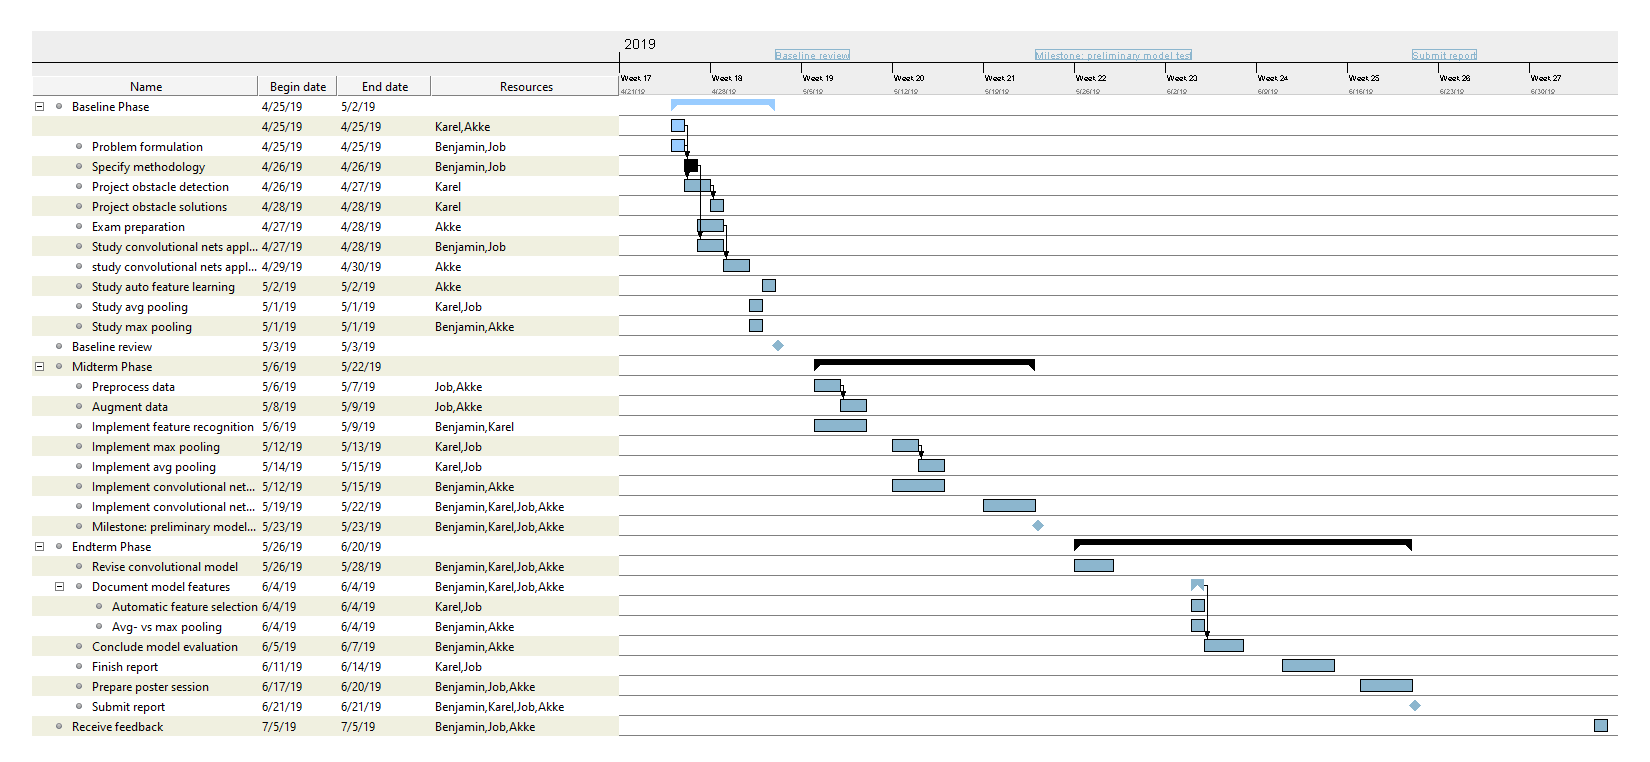
\includegraphics[width = 775pt]{images/ganttV4horizontal.png}
    \caption{Property profile of the diverse library compared to the compound pool.}
    \label{fig:PropProf}
\end{sidewaysfigure}

\subsection{Full page figure}
Figure will fill the page until the edge of the A4 that it encounters.
%\usepackage{pdfpages} % to add a full A4 size gantt chart picture
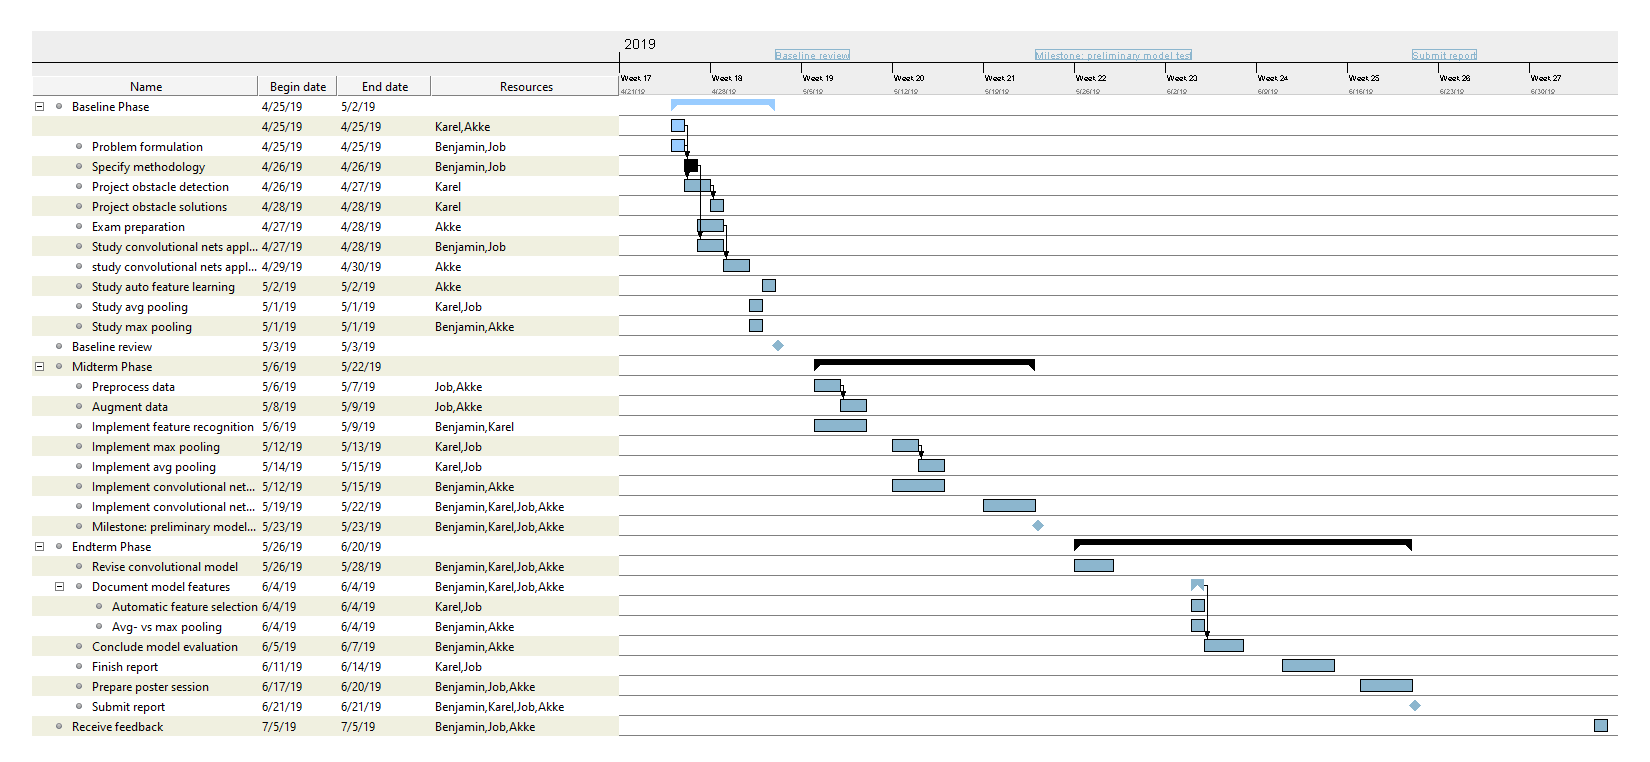
\includepdf{images/ganttV4horizontal.png}

\section{Include eps figure}
Put the following code on the top of main.tex above $begin document$ but below $documentclass{article}$.
\begin{verbatim}
\usepackage{amsmath} % need to be on top for eps files
\usepackage{graphicx}
%set the relative location for eps files
\graphicspath{ {/images/} }
\end{verbatim}

\begin{figure}
    \centering
    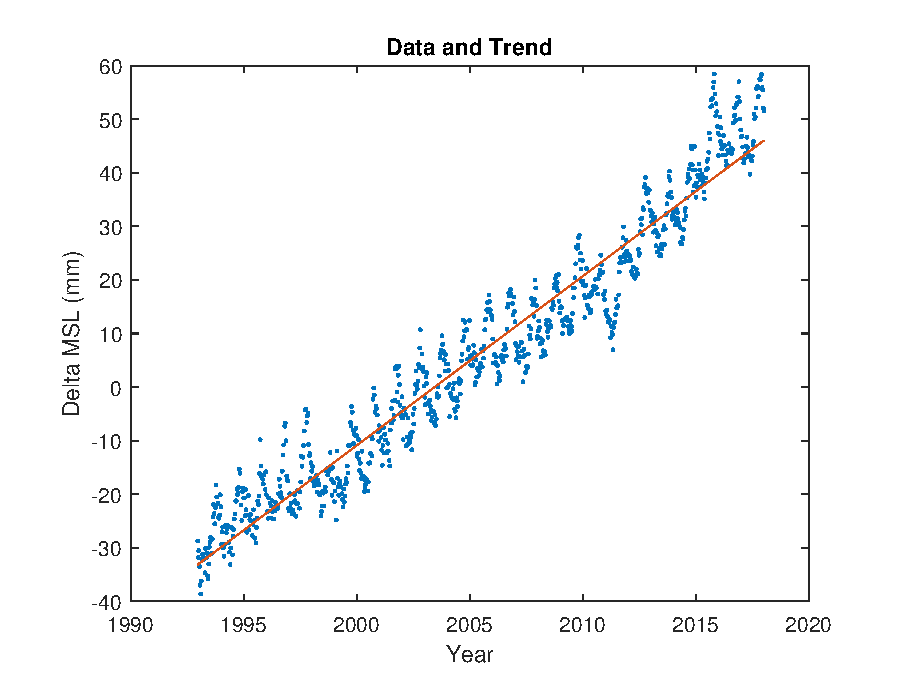
\includegraphics{images/q1a.eps}
    \caption{Trend and bias estimate and visualisation for the seasonal sea-level trend data.}
    \label{fig:plot_q1a}
\end{figure}
%Source0:https://www.latex-tutorial.com/tutorials/pgfplotstable/
%Source1:https://tex.stackexchange.com/questions/35929/using-string-variable-with-latex
% \usepackage{booktabs} % For \toprule, \midrule and \bottomrule
% \usepackage{siunitx} % Formats the units and values
% \usepackage{pgfplotstable} % Generates table from .csv

% % Setup siunitx:
% \sisetup{
%   round-mode          = places, % Rounds numbers
%   round-precision     = 2, % to 2 places
% }

% \begin{table}[h!]
% \begin{adjustwidth}{-2cm}{}
%   \begin{center}
%     \caption{Autogenerated table from .csv file.}
%     \label{table1}
%     \pgfplotstabletypeset[
%       multicolumn names, % allows to have multicolumn names
%       col sep=comma, % the seperator in our .csv file
%       display columns/0/.style={
% 		column name=$Value 1$, % name of first column
% 		column type={S},string type},  % use siunitx for formatting
%       display columns/1/.style={
% 		column name=$Value 2$,
% 		column type={S},string type},
%       every head row/.style={
% 		before row={\toprule}, % have a rule at top
% 		after row={
% 			\si{\ampere} & \si{\volt}\\ % the units seperated by &
% 			\midrule} % rule under units
% 			},
% 		every last row/.style={after row=\bottomrule}, % rule at bottom
%     ]{csvTables/table.csv} % filename/path to file
%   \end{center}
% \end{table}

\section{retry}
% Put this in Main.tex above \begin document
% \usepackage{csvsimple}
% \usepackage{geometry}
%  \geometry{
%  a4paper,
%  total={175mm,265mm},
%  left=15mm,
%  top=15mm,
%  }
 
 
\section{hi}
\hspace*{-2em}
\begin{tabular}{l|l|l|l|l|l|l|l|l}%
    \bfseries Nr. & \bfseries Cal & \bfseries tw & \bfseries Topic & \bfseries Available & \bfseries Due & \bfseries Source due & \bfseries Weight & \bfseries Source weight % specify table head
    % \csvreader[head to column names]{Basket_ball.csv}{}% use head of csv as column names
    \csvreader[head to column names]{CsvTables/table.csv}{}% use head of csv as column names
    {\\\hline\csvcoli&\csvcolii&\csvcoliii&\csvcoliv&\csvcolv&\csvcolvi&\csvcolvii&\csvcolviii&\csvcolix}% specify your coloumns here
    \end{tabular}
    


% retry try building a table from csv
% \usepackage{csvsimple}
%Source: https://tex.stackexchange.com/questions/146716/importing-csv-file-into-latex-as-a-table

% \begin{appendices}
% \crefalias{section}{appsec}
% \section{Appendix}
this is the content of the appendix.
% \section{Include PDF as appendix}\label{app:VuAB_article}
Hi this works but I did not upload the actual pdf to keep the document as short and simple as possible.
\includepdf[pages=-]{Appendices/VuAb_article.pdf}
% Insert pdf file (as appendix)
%\usepackage{pdfpages}
 
% \end{appendices}

\end{document}